% Options for packages loaded elsewhere
\PassOptionsToPackage{unicode}{hyperref}
\PassOptionsToPackage{hyphens}{url}
\PassOptionsToPackage{dvipsnames,svgnames,x11names}{xcolor}
%
\documentclass[
  letterpaper,
  DIV=11,
  numbers=noendperiod]{scrartcl}

\usepackage{amsmath,amssymb}
\usepackage{iftex}
\ifPDFTeX
  \usepackage[T1]{fontenc}
  \usepackage[utf8]{inputenc}
  \usepackage{textcomp} % provide euro and other symbols
\else % if luatex or xetex
  \usepackage{unicode-math}
  \defaultfontfeatures{Scale=MatchLowercase}
  \defaultfontfeatures[\rmfamily]{Ligatures=TeX,Scale=1}
\fi
\usepackage{lmodern}
\ifPDFTeX\else  
    % xetex/luatex font selection
\fi
% Use upquote if available, for straight quotes in verbatim environments
\IfFileExists{upquote.sty}{\usepackage{upquote}}{}
\IfFileExists{microtype.sty}{% use microtype if available
  \usepackage[]{microtype}
  \UseMicrotypeSet[protrusion]{basicmath} % disable protrusion for tt fonts
}{}
\makeatletter
\@ifundefined{KOMAClassName}{% if non-KOMA class
  \IfFileExists{parskip.sty}{%
    \usepackage{parskip}
  }{% else
    \setlength{\parindent}{0pt}
    \setlength{\parskip}{6pt plus 2pt minus 1pt}}
}{% if KOMA class
  \KOMAoptions{parskip=half}}
\makeatother
\usepackage{xcolor}
\setlength{\emergencystretch}{3em} % prevent overfull lines
\setcounter{secnumdepth}{-\maxdimen} % remove section numbering
% Make \paragraph and \subparagraph free-standing
\ifx\paragraph\undefined\else
  \let\oldparagraph\paragraph
  \renewcommand{\paragraph}[1]{\oldparagraph{#1}\mbox{}}
\fi
\ifx\subparagraph\undefined\else
  \let\oldsubparagraph\subparagraph
  \renewcommand{\subparagraph}[1]{\oldsubparagraph{#1}\mbox{}}
\fi

\usepackage{color}
\usepackage{fancyvrb}
\newcommand{\VerbBar}{|}
\newcommand{\VERB}{\Verb[commandchars=\\\{\}]}
\DefineVerbatimEnvironment{Highlighting}{Verbatim}{commandchars=\\\{\}}
% Add ',fontsize=\small' for more characters per line
\usepackage{framed}
\definecolor{shadecolor}{RGB}{241,243,245}
\newenvironment{Shaded}{\begin{snugshade}}{\end{snugshade}}
\newcommand{\AlertTok}[1]{\textcolor[rgb]{0.68,0.00,0.00}{#1}}
\newcommand{\AnnotationTok}[1]{\textcolor[rgb]{0.37,0.37,0.37}{#1}}
\newcommand{\AttributeTok}[1]{\textcolor[rgb]{0.40,0.45,0.13}{#1}}
\newcommand{\BaseNTok}[1]{\textcolor[rgb]{0.68,0.00,0.00}{#1}}
\newcommand{\BuiltInTok}[1]{\textcolor[rgb]{0.00,0.23,0.31}{#1}}
\newcommand{\CharTok}[1]{\textcolor[rgb]{0.13,0.47,0.30}{#1}}
\newcommand{\CommentTok}[1]{\textcolor[rgb]{0.37,0.37,0.37}{#1}}
\newcommand{\CommentVarTok}[1]{\textcolor[rgb]{0.37,0.37,0.37}{\textit{#1}}}
\newcommand{\ConstantTok}[1]{\textcolor[rgb]{0.56,0.35,0.01}{#1}}
\newcommand{\ControlFlowTok}[1]{\textcolor[rgb]{0.00,0.23,0.31}{#1}}
\newcommand{\DataTypeTok}[1]{\textcolor[rgb]{0.68,0.00,0.00}{#1}}
\newcommand{\DecValTok}[1]{\textcolor[rgb]{0.68,0.00,0.00}{#1}}
\newcommand{\DocumentationTok}[1]{\textcolor[rgb]{0.37,0.37,0.37}{\textit{#1}}}
\newcommand{\ErrorTok}[1]{\textcolor[rgb]{0.68,0.00,0.00}{#1}}
\newcommand{\ExtensionTok}[1]{\textcolor[rgb]{0.00,0.23,0.31}{#1}}
\newcommand{\FloatTok}[1]{\textcolor[rgb]{0.68,0.00,0.00}{#1}}
\newcommand{\FunctionTok}[1]{\textcolor[rgb]{0.28,0.35,0.67}{#1}}
\newcommand{\ImportTok}[1]{\textcolor[rgb]{0.00,0.46,0.62}{#1}}
\newcommand{\InformationTok}[1]{\textcolor[rgb]{0.37,0.37,0.37}{#1}}
\newcommand{\KeywordTok}[1]{\textcolor[rgb]{0.00,0.23,0.31}{#1}}
\newcommand{\NormalTok}[1]{\textcolor[rgb]{0.00,0.23,0.31}{#1}}
\newcommand{\OperatorTok}[1]{\textcolor[rgb]{0.37,0.37,0.37}{#1}}
\newcommand{\OtherTok}[1]{\textcolor[rgb]{0.00,0.23,0.31}{#1}}
\newcommand{\PreprocessorTok}[1]{\textcolor[rgb]{0.68,0.00,0.00}{#1}}
\newcommand{\RegionMarkerTok}[1]{\textcolor[rgb]{0.00,0.23,0.31}{#1}}
\newcommand{\SpecialCharTok}[1]{\textcolor[rgb]{0.37,0.37,0.37}{#1}}
\newcommand{\SpecialStringTok}[1]{\textcolor[rgb]{0.13,0.47,0.30}{#1}}
\newcommand{\StringTok}[1]{\textcolor[rgb]{0.13,0.47,0.30}{#1}}
\newcommand{\VariableTok}[1]{\textcolor[rgb]{0.07,0.07,0.07}{#1}}
\newcommand{\VerbatimStringTok}[1]{\textcolor[rgb]{0.13,0.47,0.30}{#1}}
\newcommand{\WarningTok}[1]{\textcolor[rgb]{0.37,0.37,0.37}{\textit{#1}}}

\providecommand{\tightlist}{%
  \setlength{\itemsep}{0pt}\setlength{\parskip}{0pt}}\usepackage{longtable,booktabs,array}
\usepackage{calc} % for calculating minipage widths
% Correct order of tables after \paragraph or \subparagraph
\usepackage{etoolbox}
\makeatletter
\patchcmd\longtable{\par}{\if@noskipsec\mbox{}\fi\par}{}{}
\makeatother
% Allow footnotes in longtable head/foot
\IfFileExists{footnotehyper.sty}{\usepackage{footnotehyper}}{\usepackage{footnote}}
\makesavenoteenv{longtable}
\usepackage{graphicx}
\makeatletter
\def\maxwidth{\ifdim\Gin@nat@width>\linewidth\linewidth\else\Gin@nat@width\fi}
\def\maxheight{\ifdim\Gin@nat@height>\textheight\textheight\else\Gin@nat@height\fi}
\makeatother
% Scale images if necessary, so that they will not overflow the page
% margins by default, and it is still possible to overwrite the defaults
% using explicit options in \includegraphics[width, height, ...]{}
\setkeys{Gin}{width=\maxwidth,height=\maxheight,keepaspectratio}
% Set default figure placement to htbp
\makeatletter
\def\fps@figure{htbp}
\makeatother

\KOMAoption{captions}{tableheading}
\makeatletter
\@ifpackageloaded{caption}{}{\usepackage{caption}}
\AtBeginDocument{%
\ifdefined\contentsname
  \renewcommand*\contentsname{Table of contents}
\else
  \newcommand\contentsname{Table of contents}
\fi
\ifdefined\listfigurename
  \renewcommand*\listfigurename{List of Figures}
\else
  \newcommand\listfigurename{List of Figures}
\fi
\ifdefined\listtablename
  \renewcommand*\listtablename{List of Tables}
\else
  \newcommand\listtablename{List of Tables}
\fi
\ifdefined\figurename
  \renewcommand*\figurename{Figure}
\else
  \newcommand\figurename{Figure}
\fi
\ifdefined\tablename
  \renewcommand*\tablename{Table}
\else
  \newcommand\tablename{Table}
\fi
}
\@ifpackageloaded{float}{}{\usepackage{float}}
\floatstyle{ruled}
\@ifundefined{c@chapter}{\newfloat{codelisting}{h}{lop}}{\newfloat{codelisting}{h}{lop}[chapter]}
\floatname{codelisting}{Listing}
\newcommand*\listoflistings{\listof{codelisting}{List of Listings}}
\makeatother
\makeatletter
\makeatother
\makeatletter
\@ifpackageloaded{caption}{}{\usepackage{caption}}
\@ifpackageloaded{subcaption}{}{\usepackage{subcaption}}
\makeatother
\ifLuaTeX
  \usepackage{selnolig}  % disable illegal ligatures
\fi
\usepackage{bookmark}

\IfFileExists{xurl.sty}{\usepackage{xurl}}{} % add URL line breaks if available
\urlstyle{same} % disable monospaced font for URLs
\hypersetup{
  pdftitle={Factors That Affect Student Performance In Exams},
  pdfauthor={Mutkallam Warraich and Jackie Yang},
  colorlinks=true,
  linkcolor={blue},
  filecolor={Maroon},
  citecolor={Blue},
  urlcolor={Blue},
  pdfcreator={LaTeX via pandoc}}

\title{Factors That Affect Student Performance In Exams}
\author{Mutkallam Warraich and Jackie Yang}
\date{2024-12-18}

\begin{document}
\maketitle

\renewcommand*\contentsname{Table of contents}
{
\hypersetup{linkcolor=}
\setcounter{tocdepth}{3}
\tableofcontents
}
\subsection{Clean Code for Research Question 1:Which gender-race
combinations show the highest vulnerability to either suicide or drug
overdose?}\label{clean-code-for-research-question-1which-gender-race-combinations-show-the-highest-vulnerability-to-either-suicide-or-drug-overdose}

\subsection{Exploratory Data Analysis (EDA) for resesarch question
one}\label{exploratory-data-analysis-eda-for-resesarch-question-one}

Suicide is a complex and deeply personal tragedy, but for some groups,
the burden is disproportionately heavy. Among American Indian or Alaska
Native males, suicide rates are the highest of any racial or gender
group, even exceeding those of White males, who also face alarmingly
high rates. This stark reality points to deeply rooted issues such as
intergenerational trauma, marginalization, and socio-economic hardships
that have plagued these communities for generations. The gender
disparity in suicide rates is clear, with males across all racial groups
more likely to take their own lives. However, American Indian or Alaska
Native females also face significant struggles, with suicide rates
higher than females in any other racial category. In contrast, Asian or
Pacific Islander males and females show the lowest suicide rates,
suggesting the potential influence of cultural or community-based
protective factors. These numbers tell a story that demands attention
and action. The high suicide rates among American Indian or Alaska
Native males highlight a desperate need for targeted mental health
support and culturally sensitive interventions. Many of these
individuals live in rural or tribal areas where access to mental health
care is severely limited, and systemic barriers only deepen the divide.
Efforts to support American Indian or Alaska Native females must also
address the stigma surrounding mental health, improve community
resources, and tackle the socio-economic challenges that
disproportionately affect these populations. To fully understand and
address these disparities, further research is needed to explore the
role of historical trauma, substance abuse, and systemic inequities in
healthcare access. The path forward requires empathy, collaboration, and
commitment. Engaging directly with tribal communities to develop mental
health programs that honor cultural values and traditions can make these
interventions more effective. Advocacy for increased funding is crucial
to ensure that mental health services reach those most in need, with a
focus on both prevention and treatment. Public health campaigns can play
a vital role in raising awareness and reducing stigma, particularly
among at-risk groups such as American Indian or Alaska Native males.
Addressing this issue is not just a matter of statistics---it is a moral
imperative to create a society where everyone, regardless of their
background, has the support they need to lead a life of hope and
purpose.

\begin{verbatim}
Warning: Removed 1600 rows containing missing values or values outside the scale range
(`geom_bar()`).
\end{verbatim}

\begin{figure}[H]

{\centering 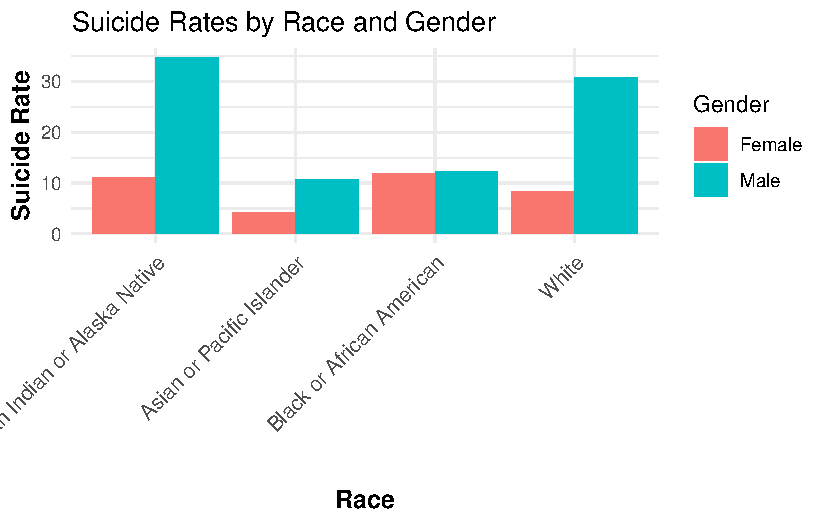
\includegraphics{Sec4_Team10_files/figure-pdf/unnamed-chunk-7-1.pdf}

}

\caption{Figure 1: Correlation Matrix}

\end{figure}%

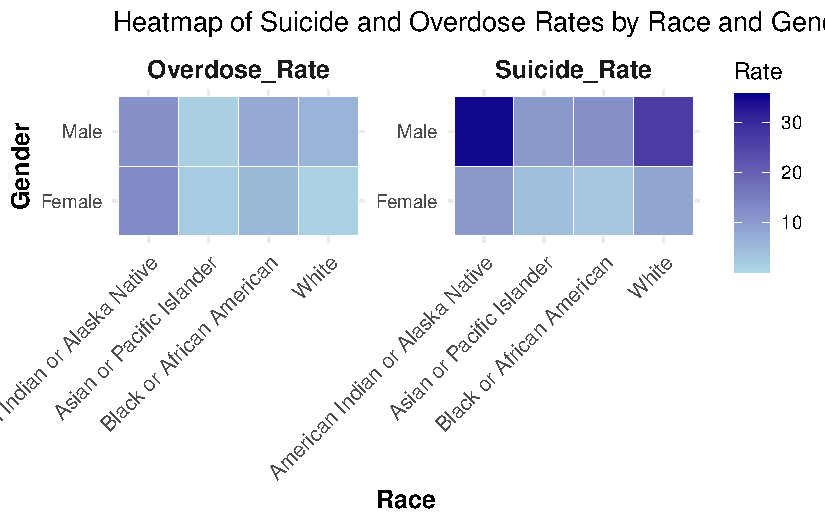
\includegraphics{Sec4_Team10_files/figure-pdf/unnamed-chunk-8-1.pdf}

This approach allowed me to analyze the data in detail, test the
hypotheses, and determine whether differences in suicide rates were
significantly influenced by ethnic, gender, or a combination of these
factors. The data, which were unequivocal and supported the rejection of
the null hypothesis, showed that there are significant differences
across gender, race, and their combinations. The alternative hypothesis
(H₁) states that there are significant differences in suicide rates,
suggesting that factors such as gender, race, or both influence the
rates displayed in the data. If at least one group shows a substantial
deviation, indicating a relationship between the observed suicide rates
and gender, race, or their interaction, the null hypothesis would be
rejected.

\begin{verbatim}
`summarise()` has grouped output by 'Race'. You can override using the
`.groups` argument.
\end{verbatim}

\begin{longtable}[]{@{}
  >{\raggedright\arraybackslash}p{(\columnwidth - 6\tabcolsep) * \real{0.3976}}
  >{\raggedright\arraybackslash}p{(\columnwidth - 6\tabcolsep) * \real{0.0843}}
  >{\raggedleft\arraybackslash}p{(\columnwidth - 6\tabcolsep) * \real{0.2530}}
  >{\raggedleft\arraybackslash}p{(\columnwidth - 6\tabcolsep) * \real{0.2651}}@{}}
\caption{Summary Table of Average Suicide and Overdose Rates by Race and
Gender}\tabularnewline
\toprule\noalign{}
\begin{minipage}[b]{\linewidth}\raggedright
Race
\end{minipage} & \begin{minipage}[b]{\linewidth}\raggedright
Gender
\end{minipage} & \begin{minipage}[b]{\linewidth}\raggedleft
Average Suicide Rate
\end{minipage} & \begin{minipage}[b]{\linewidth}\raggedleft
Average Overdose Rate
\end{minipage} \\
\midrule\noalign{}
\endfirsthead
\toprule\noalign{}
\begin{minipage}[b]{\linewidth}\raggedright
Race
\end{minipage} & \begin{minipage}[b]{\linewidth}\raggedright
Gender
\end{minipage} & \begin{minipage}[b]{\linewidth}\raggedleft
Average Suicide Rate
\end{minipage} & \begin{minipage}[b]{\linewidth}\raggedleft
Average Overdose Rate
\end{minipage} \\
\midrule\noalign{}
\endhead
\bottomrule\noalign{}
\endlastfoot
American Indian or Alaska Native & Female & 5.7458333 & 6.582609 \\
American Indian or Alaska Native & Male & 7.9946341 & 22.220652 \\
Asian or Pacific Islander & Female & 0.7960784 & 3.407500 \\
Asian or Pacific Islander & Male & 1.3919118 & 8.762500 \\
Black or African American & Female & 2.5464029 & 2.263830 \\
Black or African American & Male & 5.8938433 & 9.894444 \\
White & Female & 4.2420290 & 6.250000 \\
White & Male & 8.0163043 & 23.593478 \\
\end{longtable}

\subsection{Exploratory Data Analysis (EDA) for resesarch question
two}\label{exploratory-data-analysis-eda-for-resesarch-question-two}

The second research question, based on my topic, is: ``Is there a
significant difference in suicide rates between males and females across
racial groups?'' To answer this question, I analyzed the data in detail,
tested the hypotheses, and determined whether differences in suicide
rates were significantly influenced by ethnicity, gender, or their
combination. The approach used ensured a thorough examination of the
data, producing results that addressed the research question with
confidence. To begin, I claim the two hypotheses to guide the test. The
null hypothesis (H₀) assumed that there are no significant differences
in suicide rates across gender-race combinations, meaning that any
observed differences are purely random and there is no meanful.
Conversely, the alternative hypothesis (H₁) stated that there are
significant differences in suicide rates across these groups. This
hypothesis suggested that certain gender-race combinations might be more
vulnerable than others, indicating a relationship between the observed
suicide rates and the combination of gender and race. If at least one
group showed a substantial deviation, this would provide evidence to
reject the null hypothesis in favor of the alternative hypothesis.

The data analysis began with thorough cleaning and organization. I
started by assigning meaningful names to each group and removing
irrelevant or incomplete data that was not applicable to this research
question. Once cleaned, the dataset was categorized into three primary
components: gender (male and female), race (White, Black or African
American, American Indian or Alaska Native, and Asian or Pacific
Islander), and a gender-race combination variable. This categorization
was crucial as it allowed for a detailed examination of both the
independent effects of gender and race, as well as their interaction.
For example, while males overall might have higher suicide rates,
interaction analysis could reveal that certain racial groups within
males, such as American Indian or Alaska Native males, show
significantly higher rates than others. This organization ensured the
analysis was as thorough as possible and that no critical trends were
overlooked.And the graph is below these analyze.

Once the data was ready, I performed a Two-Way ANOVA (Analysis of
Variance) to determine whether the mean suicide rates differed
significantly by race, gender, and their interaction. The Two-Way ANOVA
is a statistical test designed to assess the effects of two independent
variables---gender and race in this case---on one dependent variable,
the suicide rates. The test addressed two primary questions: (1) whether
race and gender individually influence suicide rates (main effects), and
(2) whether the combination of gender and race creates unique patterns
that cannot be explained by their individual effects (interaction
effect). For instance, the main effect might show that males have higher
suicide rates than females, while the interaction effect could reveal
that White males or American Indian or Alaska Native males are
particularly vulnerable compared to other groups.

The results from the Two-Way ANOVA provided the first answer to my
research question by confirming that there were significant differences
in suicide rates between groups. However, while the ANOVA identified the
presence of significant differences, it could not pinpoint which
specific groups were different. To address this limitation, I used a
Tukey HSD (Honestly Significant Difference) post-hoc test, a statistical
method designed to compare the means of multiple groups while
controlling for Type I error (the risk of incorrectly identifying a
significant difference due to random chance). The Tukey HSD test builds
confidence intervals for each pairwise comparison between groups. If a
confidence interval does not include zero, it confirms that the
difference between the two groups is statistically significant. For
example, a confidence interval of {[}2.5, 7.0{]} for the difference in
suicide rates between males and females means the true difference lies
between 2.5 and 7.0, and since zero is not included, the difference is
substantial.The data is below these analyze.

The Tukey HSD test results provided detailed insights. First, in terms
of gender, the findings showed that males consistently had significantly
higher suicide rates than females. This conclusion was strongly
supported by the confidence intervals, which were all positive and
excluded zero, indicating that the difference was unlikely to be random.
Next, the analysis turned to racial groups, revealing significant
patterns. For instance, Asian or Pacific Islanders had the lowest
overall suicide rates, while American Indian or Alaska Native
individuals had the highest rates of any racial group. These findings
suggested that race alone plays a substantial role in influencing
suicide rates.

Finally, when examining the combined effects of gender and race, the
interaction analysis revealed even more pronounced disparities. White
males and American Indian or Alaska Native males had the highest suicide
rates of any group, significantly higher than groups like Asian females
and Black females, which showed the lowest rates. The Tukey HSD test
validated these findings by showing that the confidence intervals for
these comparisons did not overlap zero, confirming their statistical
significance. In summary, the statistical analysis provided compelling
evidence that gender, race, and their combination significantly
influence suicide rates. The rejection of the null hypothesis (H₀) was
supported by both the ANOVA and Tukey HSD results. Across all racial
groups, males were consistently found to be at greater risk of suicide
compared to females. Additionally, racial disparities emerged, with
American Indian or Alaska Native individuals facing the highest risk
overall. When gender and race were combined, certain groups, such as
American Indian or Alaska Native males and White males, were identified
as particularly vulnerable. These findings underscore the importance of
analyzing gender and race together, as this approach revealed patterns
that would not have been apparent if the factors were examined
independently. By following this systematic methodology, I was able to
confidently answer the research question and uncover significant
relationships within the data.

\begin{verbatim}
[1] "Tukey HSD Test Results:"
\end{verbatim}

\begin{verbatim}
  Tukey multiple comparisons of means
    95% family-wise confidence level

Fit: aov(formula = Suicide_Rate ~ Gender * Race, data = cleaned_data)

$Gender
                diff      lwr      upr p adj
Male-Female 2.610971 2.317083 2.904859     0

$Race
                                                                 diff       lwr
Asian or Pacific Islander-American Indian or Alaska Native -5.9142473 -6.517373
Black or African American-American Indian or Alaska Native -2.6509251 -3.229375
White-American Indian or Alaska Native                     -0.7351373 -1.219280
Black or African American-Asian or Pacific Islander         3.2633222  2.610875
White-Asian or Pacific Islander                             5.1791100  4.608604
White-Black or African American                             1.9157878  1.371435
                                                                  upr     p adj
Asian or Pacific Islander-American Indian or Alaska Native -5.3111217 0.0000000
Black or African American-American Indian or Alaska Native -2.0724756 0.0000000
White-American Indian or Alaska Native                     -0.2509951 0.0005586
Black or African American-Asian or Pacific Islander         3.9157692 0.0000000
White-Asian or Pacific Islander                             5.7496159 0.0000000
White-Black or African American                             2.4601410 0.0000000

$`Gender:Race`
                                                                                    diff
Male:American Indian or Alaska Native-Female:American Indian or Alaska Native  2.2488008
Female:Asian or Pacific Islander-Female:American Indian or Alaska Native      -4.9497549
Male:Asian or Pacific Islander-Female:American Indian or Alaska Native        -4.3539216
Female:Black or African American-Female:American Indian or Alaska Native      -3.1994305
Male:Black or African American-Female:American Indian or Alaska Native         0.1480100
Female:White-Female:American Indian or Alaska Native                          -1.5038043
Male:White-Female:American Indian or Alaska Native                             2.2704710
Female:Asian or Pacific Islander-Male:American Indian or Alaska Native        -7.1985557
Male:Asian or Pacific Islander-Male:American Indian or Alaska Native          -6.6027224
Female:Black or African American-Male:American Indian or Alaska Native        -5.4482313
Male:Black or African American-Male:American Indian or Alaska Native          -2.1007909
Female:White-Male:American Indian or Alaska Native                            -3.7526052
Male:White-Male:American Indian or Alaska Native                               0.0216702
Male:Asian or Pacific Islander-Female:Asian or Pacific Islander                0.5958333
Female:Black or African American-Female:Asian or Pacific Islander              1.7503244
Male:Black or African American-Female:Asian or Pacific Islander                5.0977649
Female:White-Female:Asian or Pacific Islander                                  3.4459506
Male:White-Female:Asian or Pacific Islander                                    7.2202259
Female:Black or African American-Male:Asian or Pacific Islander                1.1544911
Male:Black or African American-Male:Asian or Pacific Islander                  4.5019315
Female:White-Male:Asian or Pacific Islander                                    2.8501172
Male:White-Male:Asian or Pacific Islander                                      6.6243926
Male:Black or African American-Female:Black or African American                3.3474404
Female:White-Female:Black or African American                                  1.6956261
Male:White-Female:Black or African American                                    5.4699015
Female:White-Male:Black or African American                                   -1.6518143
Male:White-Male:Black or African American                                      2.1224611
Male:White-Female:White                                                        3.7742754
                                                                                     lwr
Male:American Indian or Alaska Native-Female:American Indian or Alaska Native  1.3770252
Female:Asian or Pacific Islander-Female:American Indian or Alaska Native      -6.0133099
Male:Asian or Pacific Islander-Female:American Indian or Alaska Native        -5.3267894
Female:Black or African American-Female:American Indian or Alaska Native      -4.1661332
Male:Black or African American-Female:American Indian or Alaska Native        -0.8290985
Female:White-Female:American Indian or Alaska Native                          -2.3195500
Male:White-Female:American Indian or Alaska Native                             1.4547254
Female:Asian or Pacific Islander-Male:American Indian or Alaska Native        -8.2503460
Male:Asian or Pacific Islander-Male:American Indian or Alaska Native          -7.5627148
Female:Black or African American-Male:American Indian or Alaska Native        -6.4019754
Male:Black or African American-Male:American Indian or Alaska Native          -3.0650805
Female:White-Male:American Indian or Alaska Native                            -4.5529517
Male:White-Male:American Indian or Alaska Native                              -0.7786763
Male:Asian or Pacific Islander-Female:Asian or Pacific Islander               -0.5411548
Female:Black or African American-Female:Asian or Pacific Islander              0.6186070
Male:Black or African American-Female:Asian or Pacific Islander                3.9571461
Female:White-Female:Asian or Pacific Islander                                  2.4401120
Male:White-Female:Asian or Pacific Islander                                    6.2143874
Female:Black or African American-Male:Asian or Pacific Islander                0.1075398
Male:Black or African American-Male:Asian or Pacific Islander                  3.4453646
Female:White-Male:Asian or Pacific Islander                                    1.9407033
Male:White-Male:Asian or Pacific Islander                                      5.7149787
Male:Black or African American-Female:Black or African American                2.2965474
Female:White-Female:Black or African American                                  0.7928104
Male:White-Female:Black or African American                                    4.5670858
Female:White-Male:Black or African American                                   -2.5657633
Male:White-Male:Black or African American                                      1.2085120
Male:White-Female:White                                                        3.0353553
                                                                                     upr
Male:American Indian or Alaska Native-Female:American Indian or Alaska Native  3.1205764
Female:Asian or Pacific Islander-Female:American Indian or Alaska Native      -3.8861999
Male:Asian or Pacific Islander-Female:American Indian or Alaska Native        -3.3810537
Female:Black or African American-Female:American Indian or Alaska Native      -2.2327277
Male:Black or African American-Female:American Indian or Alaska Native         1.1251184
Female:White-Female:American Indian or Alaska Native                          -0.6880587
Male:White-Female:American Indian or Alaska Native                             3.0862167
Female:Asian or Pacific Islander-Male:American Indian or Alaska Native        -6.1467654
Male:Asian or Pacific Islander-Male:American Indian or Alaska Native          -5.6427300
Female:Black or African American-Male:American Indian or Alaska Native        -4.4944871
Male:Black or African American-Male:American Indian or Alaska Native          -1.1365012
Female:White-Male:American Indian or Alaska Native                            -2.9522586
Male:White-Male:American Indian or Alaska Native                               0.8220167
Male:Asian or Pacific Islander-Female:Asian or Pacific Islander                1.7328215
Female:Black or African American-Female:Asian or Pacific Islander              2.8820419
Male:Black or African American-Female:Asian or Pacific Islander                6.2383836
Female:White-Female:Asian or Pacific Islander                                  4.4517891
Male:White-Female:Asian or Pacific Islander                                    8.2260644
Female:Black or African American-Male:Asian or Pacific Islander                2.2014424
Male:Black or African American-Male:Asian or Pacific Islander                  5.5584985
Female:White-Male:Asian or Pacific Islander                                    3.7595312
Male:White-Male:Asian or Pacific Islander                                      7.5338065
Male:Black or African American-Female:Black or African American                4.3983334
Female:White-Female:Black or African American                                  2.5984418
Male:White-Female:Black or African American                                    6.3727172
Female:White-Male:Black or African American                                   -0.7378653
Male:White-Male:Black or African American                                      3.0364101
Male:White-Female:White                                                        4.5131954
                                                                                  p adj
Male:American Indian or Alaska Native-Female:American Indian or Alaska Native 0.0000000
Female:Asian or Pacific Islander-Female:American Indian or Alaska Native      0.0000000
Male:Asian or Pacific Islander-Female:American Indian or Alaska Native        0.0000000
Female:Black or African American-Female:American Indian or Alaska Native      0.0000000
Male:Black or African American-Female:American Indian or Alaska Native        0.9998093
Female:White-Female:American Indian or Alaska Native                          0.0000007
Male:White-Female:American Indian or Alaska Native                            0.0000000
Female:Asian or Pacific Islander-Male:American Indian or Alaska Native        0.0000000
Male:Asian or Pacific Islander-Male:American Indian or Alaska Native          0.0000000
Female:Black or African American-Male:American Indian or Alaska Native        0.0000000
Male:Black or African American-Male:American Indian or Alaska Native          0.0000000
Female:White-Male:American Indian or Alaska Native                            0.0000000
Male:White-Male:American Indian or Alaska Native                              1.0000000
Male:Asian or Pacific Islander-Female:Asian or Pacific Islander               0.7572085
Female:Black or African American-Female:Asian or Pacific Islander             0.0000763
Male:Black or African American-Female:Asian or Pacific Islander               0.0000000
Female:White-Female:Asian or Pacific Islander                                 0.0000000
Male:White-Female:Asian or Pacific Islander                                   0.0000000
Female:Black or African American-Male:Asian or Pacific Islander               0.0188790
Male:Black or African American-Male:Asian or Pacific Islander                 0.0000000
Female:White-Male:Asian or Pacific Islander                                   0.0000000
Male:White-Male:Asian or Pacific Islander                                     0.0000000
Male:Black or African American-Female:Black or African American               0.0000000
Female:White-Female:Black or African American                                 0.0000004
Male:White-Female:Black or African American                                   0.0000000
Female:White-Male:Black or African American                                   0.0000012
Male:White-Male:Black or African American                                     0.0000000
Male:White-Female:White                                                       0.0000000
\end{verbatim}

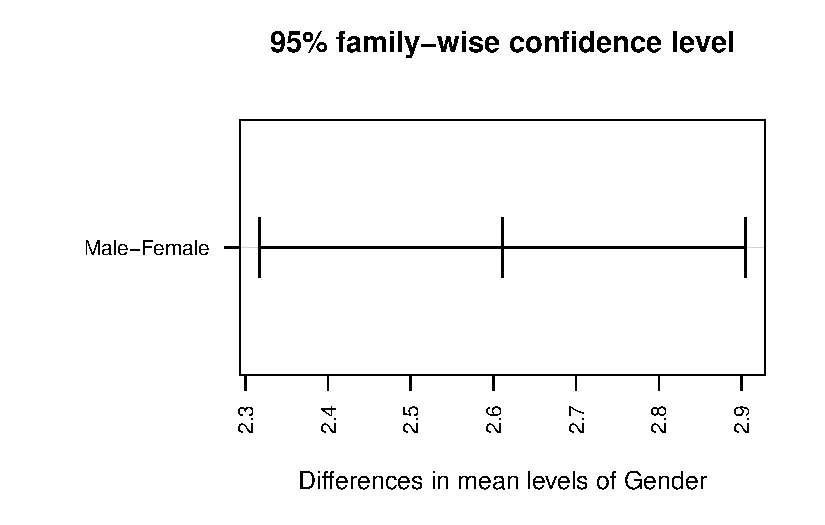
\includegraphics{Sec4_Team10_files/figure-pdf/unnamed-chunk-10-1.pdf}

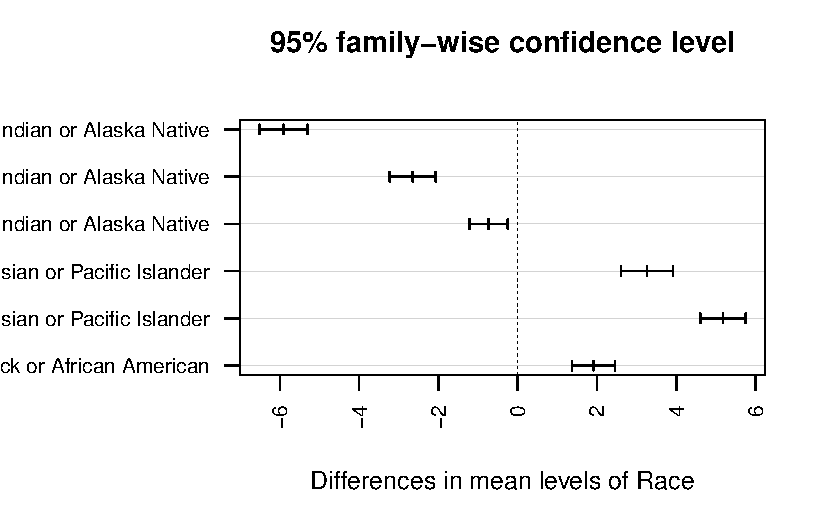
\includegraphics{Sec4_Team10_files/figure-pdf/unnamed-chunk-10-2.pdf}

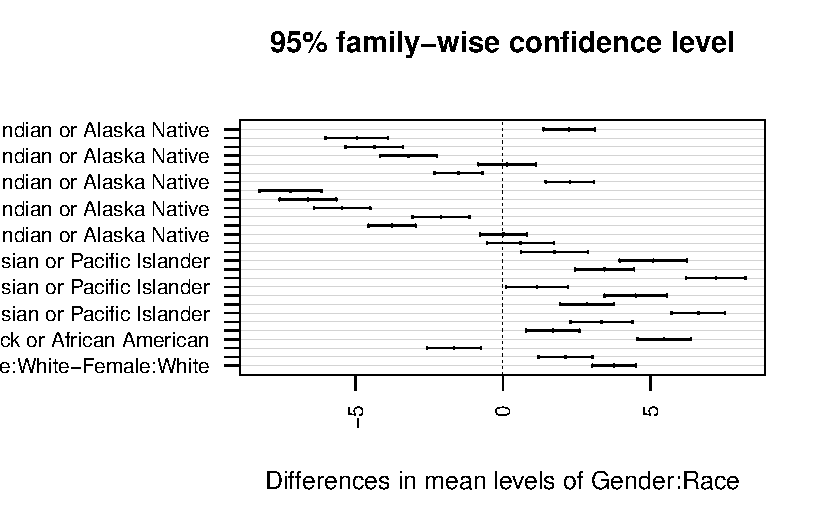
\includegraphics{Sec4_Team10_files/figure-pdf/unnamed-chunk-10-3.pdf}

\begin{Shaded}
\begin{Highlighting}[]
\CommentTok{\# This code will run, but the code and its output will be hidden.}
\FunctionTok{library}\NormalTok{(dplyr)}
\FunctionTok{library}\NormalTok{(tidyr)}
\NormalTok{suicide\_data }\OtherTok{\textless{}{-}} \FunctionTok{read.csv}\NormalTok{(}\StringTok{"https://data.cdc.gov/api/views/95ax{-}ymtc/rows.csv?accessType=DOWNLOAD"}\NormalTok{)}
\NormalTok{drug\_overdose\_data }\OtherTok{\textless{}{-}} \FunctionTok{read.csv}\NormalTok{(}\StringTok{"https://data.cdc.gov/api/views/9j2v{-}jamp/rows.csv?accessType=DOWNLOAD"}\NormalTok{)}
\CommentTok{\# Clean the suicide dataset}
\NormalTok{suicide\_clean }\OtherTok{\textless{}{-}}\NormalTok{ suicide\_data }\SpecialCharTok{\%\textgreater{}\%}
  \FunctionTok{mutate}\NormalTok{(}
    \AttributeTok{Gender =} \FunctionTok{case\_when}\NormalTok{(}
      \FunctionTok{grepl}\NormalTok{(}\StringTok{"Male"}\NormalTok{, STUB\_LABEL) }\SpecialCharTok{\textasciitilde{}} \StringTok{"Male"}\NormalTok{,}
      \FunctionTok{grepl}\NormalTok{(}\StringTok{"Female"}\NormalTok{, STUB\_LABEL) }\SpecialCharTok{\textasciitilde{}} \StringTok{"Female"}\NormalTok{,}
      \ConstantTok{TRUE} \SpecialCharTok{\textasciitilde{}} \StringTok{"All persons"}
\NormalTok{    ),}
    \AttributeTok{Race =} \FunctionTok{case\_when}\NormalTok{(}
      \FunctionTok{grepl}\NormalTok{(}\StringTok{"White"}\NormalTok{, STUB\_LABEL) }\SpecialCharTok{\textasciitilde{}} \StringTok{"White"}\NormalTok{,}
      \FunctionTok{grepl}\NormalTok{(}\StringTok{"Black or African American"}\NormalTok{, STUB\_LABEL) }\SpecialCharTok{\textasciitilde{}} \StringTok{"Black or African American"}\NormalTok{,}
      \FunctionTok{grepl}\NormalTok{(}\StringTok{"Asian or Pacific Islander"}\NormalTok{, STUB\_LABEL) }\SpecialCharTok{\textasciitilde{}} \StringTok{"Asian or Pacific Islander"}\NormalTok{,}
      \FunctionTok{grepl}\NormalTok{(}\StringTok{"American Indian or Alaska Native"}\NormalTok{, STUB\_LABEL) }\SpecialCharTok{\textasciitilde{}} \StringTok{"American Indian or Alaska Native"}\NormalTok{,}
      \ConstantTok{TRUE} \SpecialCharTok{\textasciitilde{}} \StringTok{"Unknown"}
\NormalTok{    )}
\NormalTok{  ) }\SpecialCharTok{\%\textgreater{}\%}
  \FunctionTok{select}\NormalTok{(}
\NormalTok{    Gender, }
\NormalTok{    Race,}
    \AttributeTok{Year =}\NormalTok{ YEAR,}
    \AttributeTok{Age\_Group =}\NormalTok{ AGE,}
    \AttributeTok{Suicide\_Rate =}\NormalTok{ ESTIMATE}
\NormalTok{  ) }\SpecialCharTok{\%\textgreater{}\%}
  \FunctionTok{filter}\NormalTok{(Gender }\SpecialCharTok{!=} \StringTok{"All persons"}\NormalTok{) }\CommentTok{\# Exclude general rows if needed}

\CommentTok{\# Clean the drug overdose dataset}
\NormalTok{drug\_overdose\_clean }\OtherTok{\textless{}{-}}\NormalTok{ drug\_overdose\_data }\SpecialCharTok{\%\textgreater{}\%}
  \FunctionTok{mutate}\NormalTok{(}
    \AttributeTok{Gender =} \FunctionTok{case\_when}\NormalTok{(}
      \FunctionTok{grepl}\NormalTok{(}\StringTok{"Male"}\NormalTok{, STUB\_LABEL) }\SpecialCharTok{\textasciitilde{}} \StringTok{"Male"}\NormalTok{,}
      \FunctionTok{grepl}\NormalTok{(}\StringTok{"Female"}\NormalTok{, STUB\_LABEL) }\SpecialCharTok{\textasciitilde{}} \StringTok{"Female"}\NormalTok{,}
      \ConstantTok{TRUE} \SpecialCharTok{\textasciitilde{}} \StringTok{"All persons"}
\NormalTok{    ),}
    \AttributeTok{Race =} \FunctionTok{case\_when}\NormalTok{(}
      \FunctionTok{grepl}\NormalTok{(}\StringTok{"White"}\NormalTok{, STUB\_LABEL) }\SpecialCharTok{\textasciitilde{}} \StringTok{"White"}\NormalTok{,}
      \FunctionTok{grepl}\NormalTok{(}\StringTok{"Black or African American"}\NormalTok{, STUB\_LABEL) }\SpecialCharTok{\textasciitilde{}} \StringTok{"Black or African American"}\NormalTok{,}
      \FunctionTok{grepl}\NormalTok{(}\StringTok{"Asian or Pacific Islander"}\NormalTok{, STUB\_LABEL) }\SpecialCharTok{\textasciitilde{}} \StringTok{"Asian or Pacific Islander"}\NormalTok{,}
      \FunctionTok{grepl}\NormalTok{(}\StringTok{"American Indian or Alaska Native"}\NormalTok{, STUB\_LABEL) }\SpecialCharTok{\textasciitilde{}} \StringTok{"American Indian or Alaska Native"}\NormalTok{,}
      \ConstantTok{TRUE} \SpecialCharTok{\textasciitilde{}} \StringTok{"Unknown"}
\NormalTok{    )}
\NormalTok{  ) }\SpecialCharTok{\%\textgreater{}\%}
  \FunctionTok{select}\NormalTok{(}
\NormalTok{    Gender,}
\NormalTok{    Race,}
    \AttributeTok{Year =}\NormalTok{ YEAR,}
    \AttributeTok{Age\_Group =}\NormalTok{ AGE,}
    \AttributeTok{Overdose\_Rate =}\NormalTok{ ESTIMATE}
\NormalTok{  ) }\SpecialCharTok{\%\textgreater{}\%}
  \FunctionTok{filter}\NormalTok{(Gender }\SpecialCharTok{!=} \StringTok{"All persons"}\NormalTok{) }\CommentTok{\# Exclude general rows if needed}
\CommentTok{\# Merge the two datasets}
\NormalTok{merged\_data }\OtherTok{\textless{}{-}} \FunctionTok{merge}\NormalTok{(}
\NormalTok{  suicide\_clean,}
\NormalTok{  drug\_overdose\_clean,}
  \AttributeTok{by =} \FunctionTok{c}\NormalTok{(}\StringTok{"Gender"}\NormalTok{, }\StringTok{"Race"}\NormalTok{, }\StringTok{"Year"}\NormalTok{, }\StringTok{"Age\_Group"}\NormalTok{),}
  \AttributeTok{all =} \ConstantTok{FALSE} 
\NormalTok{)}

\NormalTok{merged\_data }\OtherTok{\textless{}{-}}\NormalTok{ merged\_data }\SpecialCharTok{\%\textgreater{}\%}
  \FunctionTok{filter}\NormalTok{(Race }\SpecialCharTok{!=} \StringTok{"Unknown"}\NormalTok{) }\SpecialCharTok{\%\textgreater{}\%} \CommentTok{\# Remove rows with unknown race}
  \FunctionTok{select}\NormalTok{(}\SpecialCharTok{{-}}\NormalTok{Age\_Group, }\SpecialCharTok{{-}}\NormalTok{Year)     }\CommentTok{\# Drop the Age\_Group and Year columns entirely}

\FunctionTok{write.csv}\NormalTok{(merged\_data, }\StringTok{"Cleaned\_Combined\_Death\_Rates.csv"}\NormalTok{, }\AttributeTok{row.names =} \ConstantTok{FALSE}\NormalTok{)}
\FunctionTok{write.csv}\NormalTok{(}
\NormalTok{  merged\_data,}
  \StringTok{"C:/Users/hanzi/Downloads/Cleaned\_Combined\_Death\_Rates.csv"}\NormalTok{,}
  \AttributeTok{row.names =} \ConstantTok{FALSE}
\NormalTok{)}
\DocumentationTok{\#\# Image 1 for Question 1}
\FunctionTok{library}\NormalTok{(ggplot2)}
\CommentTok{\# Bar chart: Death rates by gender and race}
\FunctionTok{ggplot}\NormalTok{(}\AttributeTok{data =}\NormalTok{ merged\_data, }\FunctionTok{aes}\NormalTok{(}\AttributeTok{x =}\NormalTok{ Race, }\AttributeTok{y =}\NormalTok{ Suicide\_Rate, }\AttributeTok{fill =}\NormalTok{ Gender)) }\SpecialCharTok{+}
  \FunctionTok{geom\_bar}\NormalTok{(}\AttributeTok{stat =} \StringTok{"identity"}\NormalTok{, }\AttributeTok{position =} \StringTok{"dodge"}\NormalTok{) }\SpecialCharTok{+}
  \FunctionTok{theme\_minimal}\NormalTok{() }\SpecialCharTok{+}
  \FunctionTok{theme}\NormalTok{(}
    \AttributeTok{axis.text.x =} \FunctionTok{element\_text}\NormalTok{(}\AttributeTok{angle =} \DecValTok{45}\NormalTok{, }\AttributeTok{hjust =} \DecValTok{1}\NormalTok{, }\AttributeTok{size =} \DecValTok{10}\NormalTok{),}
    \AttributeTok{axis.title.x =} \FunctionTok{element\_text}\NormalTok{(}\AttributeTok{size =} \DecValTok{12}\NormalTok{, }\AttributeTok{face =} \StringTok{"bold"}\NormalTok{),}
    \AttributeTok{axis.title.y =} \FunctionTok{element\_text}\NormalTok{(}\AttributeTok{size =} \DecValTok{12}\NormalTok{, }\AttributeTok{face =} \StringTok{"bold"}\NormalTok{)}
\NormalTok{  ) }\SpecialCharTok{+}
  \FunctionTok{labs}\NormalTok{(}
    \AttributeTok{title =} \StringTok{"Suicide Rates by Race and Gender"}\NormalTok{,}
    \AttributeTok{x =} \StringTok{"Race"}\NormalTok{,}
    \AttributeTok{y =} \StringTok{"Suicide Rate"}\NormalTok{,}
    \AttributeTok{fill =} \StringTok{"Gender"}
\NormalTok{  )}
\DocumentationTok{\#\# Image 2 for Question 1}
\CommentTok{\# Load required library}
\FunctionTok{library}\NormalTok{(tidyr)}

\CommentTok{\# Transform data to long format}
\NormalTok{merged\_data\_long }\OtherTok{\textless{}{-}}\NormalTok{ merged\_data }\SpecialCharTok{\%\textgreater{}\%}
  \FunctionTok{pivot\_longer}\NormalTok{(}\AttributeTok{cols =} \FunctionTok{c}\NormalTok{(Suicide\_Rate, Overdose\_Rate), }
               \AttributeTok{names\_to =} \StringTok{"Variable"}\NormalTok{, }
               \AttributeTok{values\_to =} \StringTok{"Rate"}\NormalTok{)}

\CommentTok{\# Heatmap: Combined rates by race and gender}
\FunctionTok{library}\NormalTok{(ggplot2)}

\FunctionTok{ggplot}\NormalTok{(}\AttributeTok{data =}\NormalTok{ merged\_data\_long, }\FunctionTok{aes}\NormalTok{(}\AttributeTok{x =}\NormalTok{ Race, }\AttributeTok{y =}\NormalTok{ Gender, }\AttributeTok{fill =}\NormalTok{ Rate)) }\SpecialCharTok{+}
  \FunctionTok{geom\_tile}\NormalTok{(}\AttributeTok{color =} \StringTok{"white"}\NormalTok{) }\SpecialCharTok{+}
  \FunctionTok{facet\_wrap}\NormalTok{(}\SpecialCharTok{\textasciitilde{}}\NormalTok{ Variable, }\AttributeTok{scales =} \StringTok{"free"}\NormalTok{, }\AttributeTok{ncol =} \DecValTok{2}\NormalTok{) }\SpecialCharTok{+} \CommentTok{\# Adjust facets}
  \FunctionTok{scale\_fill\_gradient}\NormalTok{(}\AttributeTok{low =} \StringTok{"lightblue"}\NormalTok{, }\AttributeTok{high =} \StringTok{"darkblue"}\NormalTok{, }\AttributeTok{name =} \StringTok{"Rate"}\NormalTok{) }\SpecialCharTok{+}
  \FunctionTok{theme\_minimal}\NormalTok{() }\SpecialCharTok{+}
  \FunctionTok{theme}\NormalTok{(}
    \AttributeTok{axis.text.x =} \FunctionTok{element\_text}\NormalTok{(}\AttributeTok{angle =} \DecValTok{45}\NormalTok{, }\AttributeTok{hjust =} \DecValTok{1}\NormalTok{, }\AttributeTok{size =} \DecValTok{10}\NormalTok{), }\CommentTok{\# Rotate and space x{-}axis labels}
    \AttributeTok{axis.title.x =} \FunctionTok{element\_text}\NormalTok{(}\AttributeTok{size =} \DecValTok{12}\NormalTok{, }\AttributeTok{face =} \StringTok{"bold"}\NormalTok{),}
    \AttributeTok{axis.title.y =} \FunctionTok{element\_text}\NormalTok{(}\AttributeTok{size =} \DecValTok{12}\NormalTok{, }\AttributeTok{face =} \StringTok{"bold"}\NormalTok{),}
    \AttributeTok{strip.text =} \FunctionTok{element\_text}\NormalTok{(}\AttributeTok{size =} \DecValTok{12}\NormalTok{, }\AttributeTok{face =} \StringTok{"bold"}\NormalTok{) }\CommentTok{\# For facet titles}
\NormalTok{  ) }\SpecialCharTok{+}
  \FunctionTok{labs}\NormalTok{(}
    \AttributeTok{title =} \StringTok{"Heatmap of Suicide and Overdose Rates by Race and Gender"}\NormalTok{,}
    \AttributeTok{x =} \StringTok{"Race"}\NormalTok{,}
    \AttributeTok{y =} \StringTok{"Gender"}
\NormalTok{  )}
\DocumentationTok{\#\# Image 3 for Question 1}
\CommentTok{\# Summarize the data by Race and Gender}
\NormalTok{summary\_table }\OtherTok{\textless{}{-}}\NormalTok{ merged\_data }\SpecialCharTok{\%\textgreater{}\%}
  \FunctionTok{group\_by}\NormalTok{(Race, Gender) }\SpecialCharTok{\%\textgreater{}\%}
  \FunctionTok{summarise}\NormalTok{(}
    \AttributeTok{Avg\_Suicide\_Rate =} \FunctionTok{mean}\NormalTok{(Suicide\_Rate, }\AttributeTok{na.rm =} \ConstantTok{TRUE}\NormalTok{),}
    \AttributeTok{Avg\_Overdose\_Rate =} \FunctionTok{mean}\NormalTok{(Overdose\_Rate, }\AttributeTok{na.rm =} \ConstantTok{TRUE}\NormalTok{)}
\NormalTok{  )}

\CommentTok{\# Display the summary table}
\FunctionTok{library}\NormalTok{(knitr)}
\FunctionTok{kable}\NormalTok{(summary\_table, }
      \AttributeTok{col.names =} \FunctionTok{c}\NormalTok{(}\StringTok{"Race"}\NormalTok{, }\StringTok{"Gender"}\NormalTok{, }\StringTok{"Average Suicide Rate"}\NormalTok{, }\StringTok{"Average Overdose Rate"}\NormalTok{),}
      \AttributeTok{caption =} \StringTok{"Summary Table of Average Suicide and Overdose Rates by Race and Gender"}\NormalTok{)}
\CommentTok{\# Step 1: Load the dataset}
\NormalTok{data }\OtherTok{\textless{}{-}} \FunctionTok{read.csv}\NormalTok{(}\StringTok{"Cleaned\_Combined\_Death\_Rates.csv"}\NormalTok{)}

\CommentTok{\# Step 2: Clean the data}
\CommentTok{\# Select relevant columns and remove rows with missing values}
\NormalTok{cleaned\_data }\OtherTok{\textless{}{-}}\NormalTok{ data }\SpecialCharTok{\%\textgreater{}\%}
  \FunctionTok{select}\NormalTok{(Gender, Race, Suicide\_Rate) }\SpecialCharTok{\%\textgreater{}\%}
  \FunctionTok{na.omit}\NormalTok{()}

\CommentTok{\# Step 3: Perform Two{-}Way ANOVA}
\CommentTok{\# Test for differences in suicide rates between gender and racial groups}
\NormalTok{anova\_model }\OtherTok{\textless{}{-}} \FunctionTok{aov}\NormalTok{(Suicide\_Rate }\SpecialCharTok{\textasciitilde{}}\NormalTok{ Gender }\SpecialCharTok{*}\NormalTok{ Race, }\AttributeTok{data =}\NormalTok{ cleaned\_data)}

\CommentTok{\# Step 5: Perform Post{-}hoc Tukey HSD test}
\NormalTok{tukey\_results }\OtherTok{\textless{}{-}} \FunctionTok{TukeyHSD}\NormalTok{(anova\_model)}
\FunctionTok{print}\NormalTok{(}\StringTok{"Tukey HSD Test Results:"}\NormalTok{)}
\FunctionTok{print}\NormalTok{(tukey\_results)}

\CommentTok{\# Step 6: Adjust graphical parameters for better margins and readability}
\FunctionTok{par}\NormalTok{(}\AttributeTok{cex.axis =} \FloatTok{0.6}\NormalTok{)        }\CommentTok{\# Reduce axis text size}
\FunctionTok{par}\NormalTok{(}\AttributeTok{las =} \DecValTok{2}\NormalTok{)      }\CommentTok{\# Rotate axis labels}

\FunctionTok{par}\NormalTok{(}\AttributeTok{mar =} \FunctionTok{c}\NormalTok{(}\DecValTok{5}\NormalTok{, }\DecValTok{8}\NormalTok{, }\DecValTok{4}\NormalTok{, }\DecValTok{2}\NormalTok{))  }\CommentTok{\# Increase left margin for better label visibility}
\FunctionTok{plot}\NormalTok{(tukey\_results, }\AttributeTok{las =} \DecValTok{2}\NormalTok{, }\AttributeTok{cex.axis =} \FloatTok{0.8}\NormalTok{)  }\CommentTok{\# Rotate axis labels and adjust size}
\CommentTok{\# Step 7: Plot Tukey HSD results}
\end{Highlighting}
\end{Shaded}




\end{document}
